%!TEX root = ../../main.tex

\chapter{EDRICO}

The Proposed Processor design named Educational DHBW RISC-V Core (EDRICO) implements a basic RV32I
instruction set architecture. Besides the mandatory “Zicsr” extension no other
instruction set extensions are implemented. To keep the implementation simple and
straight-forward only one privilege mode (Machine-mode) is implemented. This mode
allows full access to the processor and peripherals. Future Versions could be
extended to implement Supervisor-Mode and User-Mode.\\
The core is a simple \acf{SISD} processor without any pipeline or cache. The basic instruction cycle of fetch, decode, execute, store is performed for every instruction one at a time.\\
Figure \ref{fig:edricooverview} shows the full overview of the processor design:

\begin{figure}[H]
	\centering
	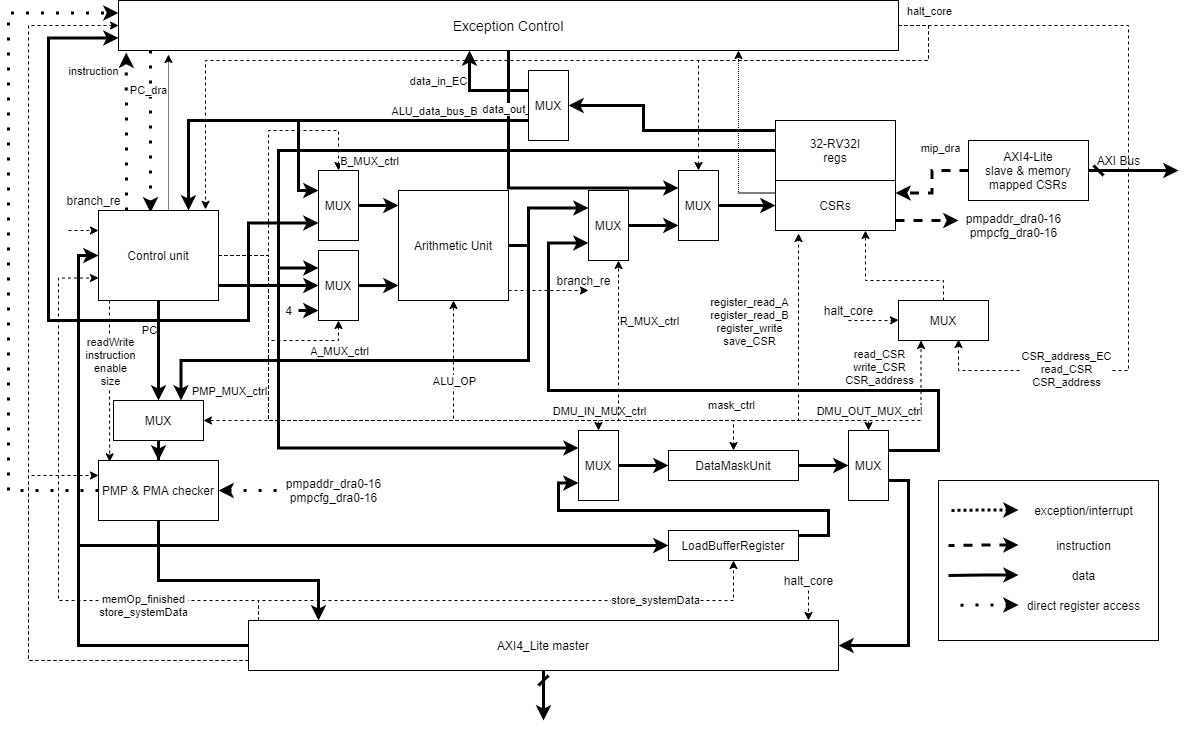
\includegraphics[width=150mm,scale=0.5]{datapath_EDRICO}
	\caption{EDRICO Overview}
	\label{fig:edricooverview}
\end{figure}

Its main components are the Exception Control, Control Unit, Arithmetic Unit,
Register Files, PMP \& PMA checker and the AXI4 Interfaces. How these components interact with each other, in order to execute Instructions, is specified in the Data Path.
The following sections will describe each one of the sections in more detail.

\section{Data Path}
The Data Path specifies how the data is passed through the Processor Core at run time. It therefore determines what registers are read and written at which clock cycle, what control signals need to be applied and how many cycles the instruction execution takes.\\
To run an instruction, it must be fetched, decoded and executed. Execution varies for different instructions.\\
To perform for example a load, the target address must be calculated and verified for possible access constraints. After successfully accessing the memory space, the obtained data is modified to satisfy the instruction specific formatting. 
A load half-word unsigned operation for instance must return a 32-Bit value by zero extending the loaded two bytes of data.\\
In case of a simple register-register addition, execution is found to be a lot simpler. Addition is performed inside the Arithmetic Logic Unit on two register values. The result is stored to the target register on the next falling clock edge.\\
With the end of the execute phase, the Programm Counter is updated. This ensures that the 32-Bit register always contains the address of the current instruction to be fetched, decoded and executed.  \\
Figure \ref{fig:datapath_generic} shows the different actions that are performed on each clock cycles during run time:

\begin{figure}[H]
	\centering
	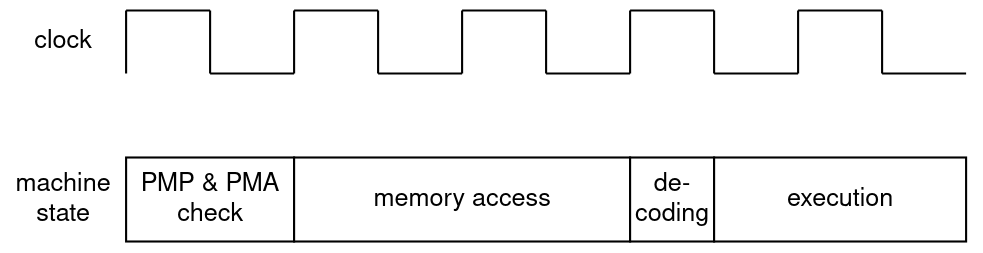
\includegraphics[width=150mm,scale=0.5]{DataPath}
	\caption{Generic Data Path}
	\label{fig:datapath_generic}
\end{figure}

Prior to memory access, the address must be checked for possible violations of the physical memory protection (PMP) and physical memory attribute (PMA) rules. Therefore the PC is passed to the PMP and PMA checker unit (see: \ref{fig:edricooverview}).\\
PMP and PMA checks are finished one clock cycle later, if an exception is generated, the trap is taken. Otherwise the data as well as the control signals are passed to the AXI4-Lite master.
The AXI4-Lite transfer will take multiple clock cycles. Its length can be increased by external factors, such as the memory to be accessed or the amount of data currently passing through the AXI-interconnect. To simplify the depiction in \ref{fig:datapath_generic} it is assumed to take only two clock cycles.\\
After successfully accessing the memory, decoding is performed in half a clock cycle. Decoding returns all the control signals of EDRICO set to the correct levels in order to perform the desired operation. Hence, no control signals do change during execution. This is desired since it will allow an easier pipelined implementation of a RISC-V core based on EDRICO.\\
Execution is displayed to take one and a half clock cycles. The registers are written at the falling clock cycle, one cycle after decoding started. Therefore execution is finished after only one clock cycle and not one and a half. Since the next instruction fetch is issued at a rising clock edge the machine must remain in execution state for an additional half clock cycle. \\
The fact that some registers are falling-edge and others rising-edge sensitive may seem a little bit disturbing at first glance. It is done to allow easier implementation and achieving of timing-closure during place and rout. If, for example, a critical path is found to be at the decode process, the duty cycle of the clock can be modified in order to achieve a higher possible clock frequency.


\section{Control Unit}
The \ac{CU} is the heart of the processor and controls the other parts of the processor depending on the input instruction. The CU is responsible for fetching instructions from the instruction memory, decode the bitstream and set the respective control signals for the other processor components. Due to the complexity of the CU, there are several sub-modules which together form the overall CU.
\subsection{Architecture and Design}
\label{CU_arch}
A general overview of the CU architecture is displayed in Figure \ref{fig:cuarchitecture}. 

\begin{figure}[H]
	\centering
	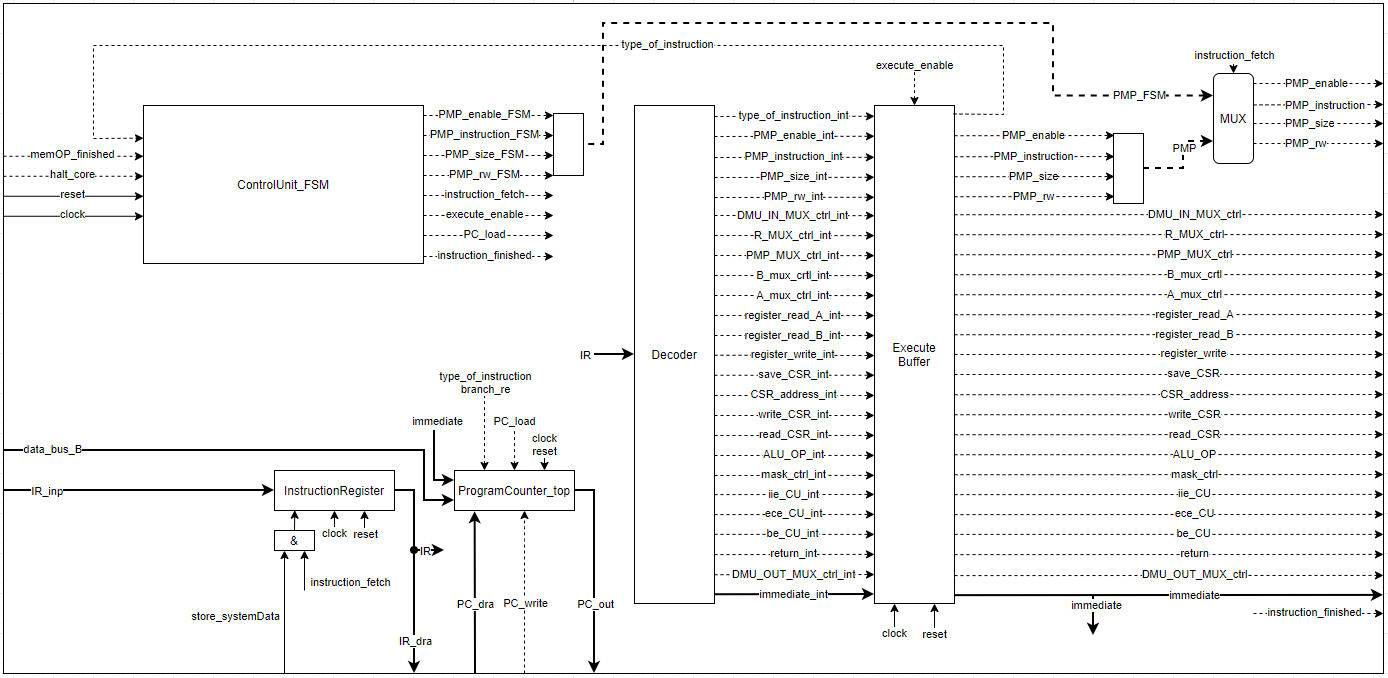
\includegraphics[width=\textwidth]{CU_architecture}
	\caption{Control Unit Architecture}
	\label{fig:cuarchitecture}
\end{figure}

To describe the functionality of the CU in more detail, every sub-module will be described closely.\\
Since the Control Unit is responsible for the whole processor, it is important to have a persistent and stable procedure for every instruction that shall be executed. The Control Unit \ac{FSM} is responsible for the correct clock timings which is important due to memory operations and the execution time of the other processor parts. The states and conditions of the FSM are displayed in Figure \ref{fig:cufsm}. 

\begin{figure}[H]
	\centering
	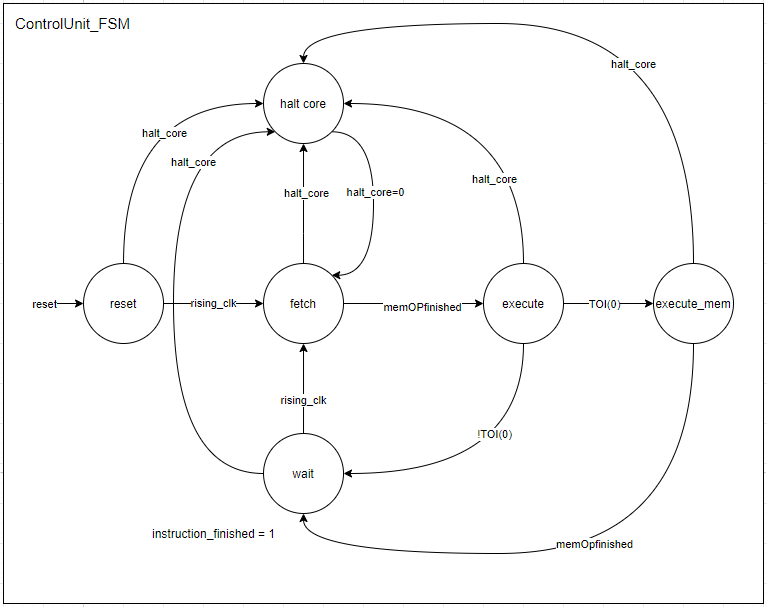
\includegraphics[width=\textwidth]{CU_FSM}
	\caption{Control Unit FSM overview}
	\label{fig:cufsm}
\end{figure}

Table \ref{tableFSM} shows a more detailed overview of the clock cycles and the corresponding actions and states:\\

\begin{table}[h]
\setlength\arrayrulewidth{2pt}	
\resizebox{\textwidth}{!}{
	\begin{tabular}{|c|c|l|l|}
		\hline
		\rowcolor{light-gray}
		\textbf{ClockCycle} & \textbf{Edge} & \textbf{Action} & \textbf{Signal} \\
		\hline
		1 & rising & pass the PC and enable PMP \& PMA checker with respective information &  \\
		\hline
		& falling & N/A &  \\
		\hline
		4 & rising & data is ready in instruction register - switch to execute state & \textit{memOPfinished} \& \textit{store\_systemData} is high \\
		\hline
		5 & rising & execution is started - if memory operation wait for another \textit{memOPfinished} flag, otherwise wait & \textit{execute\_enable} \\
		\hline
		x & rising & during memory operation: data loaded to buffer \textbackslash store transfer finished $\rightarrow$ wait state & \textit{memOPfinished} \& \textit{store\_systemData} is high \\
		\hline
		& falling & if load: store data form buffer to specified location &  \\
		\hline
		6 / x+1 & rising & go to \textit{fetch\_state} &  \\
		\hline
	\end{tabular}}
\caption{Timing of FSM}
\label{tableFSM}
\end{table}

During an execution cycle, the FSM controls the rest of the CU consisting of memory, decoding unit, PC control and the different multiplexers. To understand what the purpose of the different signals are, the other components of the Control Unit are described in the following sections.

After loading an instruction from the memory to the instruction register, the decoding process can begin. The responsible part for this process is the decoding unit which is described below.(Also visible in figure \ref{fig:cuarchitecture})\\
In this project the RISC-V RS32I instruction set is used which consists of 32-bit instruction words. The instruction words have a pre-defined structure and are divided into six instruction formats.
The instruction formats are shown in Figure \ref{fig:instrtypes}.

\begin{figure}[h]
	\centering
	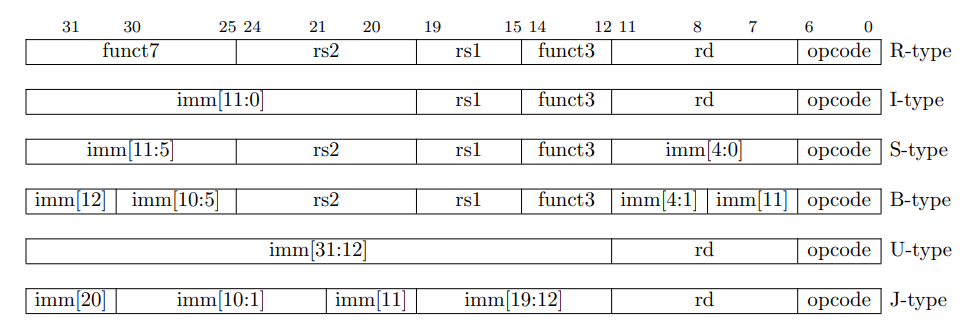
\includegraphics[width=\textwidth]{instr_types.png}
	\caption{RISC-V Instruction formats \cite{riscv}}
	\label{fig:instrtypes}
\end{figure}
The different instruction formats are useful for the decoding process since e.g. all LOAD instructions have the same structure and therefore, the effort to decode the 32-bit word can be reduced. Since the control signals are unique for every instruction and depending on the content of the 32-bit word, the decoder has to identify the encoded instruction, extract the information and respectively set the control signals, calculate immediates and control the multiplexers. A more detailed description of the decoding process can be found in section \ref{CU_impl}.\\
After the instruction is decoded, all output control signals are stable and ready to be fed through. Before leaving the CU, the \textit{Execute Buffer} (figure \ref{fig:cuarchitecture}) buffers the control signals. Once the FSM sets the \textit{execute\_enable} flag, the control signals are fed through. This buffer prevents the processor to confuse timing and clock cycles, or use signals which are not yet set correctly.\\
During an instruction execution, the program counter has to be incremented for the processor to know what instruction will follow. \textit{But} since there are several instructions that modify the program counter, a so called \textit{PC control} is designed. The PC control receives information from the decoder which consists of a 4 bit signal. The different instructions and the respective action as well as the respective control signal are shown in following table \ref{PCcontrol}:\clearpage

\begin{table}[h]
\setlength\arrayrulewidth{2pt}
	\resizebox{\textwidth}{!}{
		\begin{tabular}{|l|l|l|}
			\hline
			\rowcolor{light-gray}
			\textbf{Instruction} & \textbf{Action} & \textbf{Control Signal}\\
			\hline
			Default & No action required & \textbf{0000}\\
			\hline
			Branch & Depending on the result of branch operation, PC will be incremented respectively & \textbf{0010}\\
			\hline
			JAL & Target address obtained by adding current PC and immediate, rejump address stored in register & \textbf{0100}\\
			\hline
			JALR & Target address obtained by adding input register to immediate & \textbf{1000}\\
			\hline
		\end{tabular}}
	\label{PCcontrol}
	\caption{Program Counter control: Instructions and resulting actions}
\end{table}
For instructions which do not influence the program counter, the standard operation performs the \textbf{PC + 4} operation.

The instruction register displayed in figure \ref{fig:cuarchitecture} manages the instruction string coming from the memory.
All of these parts together form the Control Unit and are responsible for the correct execution of the instructions. The implementation of the sub-units in VHDL are described in the following section \ref{CU_impl}.\clearpage

\subsection{Implementation}
\label{CU_impl}
The implementation of the Control Unit is split up into multiple sub-implementations. As shown in figure \ref{fig:cuarchitecture} those sub-modules are the \textit{FSM, decoder, execute\_buffer, PC control and instruction register}. Since the implementation of the FSM is very similar to other FSM implementations in this project, the detailed description of a FSM in VHDL is found in the next chapters.\\
In this section the implementation of the decoder will be described more closely.
As already described in section \ref{CU_arch} the instructions can be separated in different instruction formats. To distinguish the different instructions, so-called \textit{instruction clusters} are created. These clusters sum up instructions which are encoded in the same instruction format or in general are similar.
The following table shows the different clusters and the corresponding instructions:
\begin{table}[h]
\setlength\arrayrulewidth{2pt}
	\centering
		\begin{tabular}{|l|l|}
			\hline
			\rowcolor{light-gray}
			\textbf{Cluster} & \textbf{Instructions}\\
		
			\hline
			LOAD & Load - Byte \textbackslash Halfword \textbackslash Word\\
			
			\hline
			STORE & Store - Byte \textbackslash Halfword \textbackslash Word\\
			
			\hline
			BRANCH & Different Branch Instructions (e.b. Branch if equal)\\
			
			\hline
			JALR & only JALR, since it has a unique instruction structure\\
			
			\hline
			JAL & only JAL, since it has a unique instruction structure\\
			
			\hline
			OP & All arithmetic instructions like ADD, SUB, shift and comparisons\\
			
			\hline
			OP-IMM & All arithmetic instructions performed with immediate\\
			\hline
			AUIPC & only AUIPC, since it has a unique instruction structure\\
			\hline
			LUI & only LUI, since it has a unique instruction structure\\
			\hline			
	\end{tabular}
	\label{instructioncluster}
	\caption{Decoding instruction clusters}
\end{table}


To determine the cluster for each instruction, a decoding procedure is implemented in VHDL based on structure visualized in figure \ref{fig:decode_structure}:

\begin{figure}[H]
	\centering
	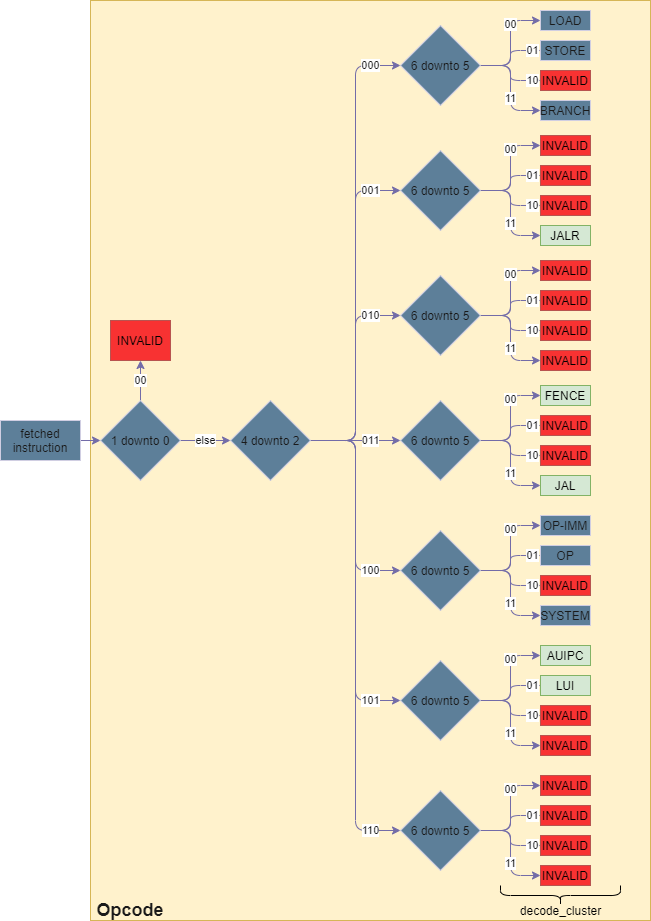
\includegraphics[width = 120mm]{Decode_Structure}
	\caption{Decoding Structure to determine instruction cluster}
	\label{fig:decode_structure}
\end{figure}
After determining the cluster, the VHDL code assigns all the outputs visible in figure \ref{fig:cuarchitecture} with the respective information. For a better understanding of the information extraction, figure \ref{fig:instruction_bits} shows how the 32-bit instruction word is split up (in this case for the \textit{OP} and \textit{OP-IMM} instructions.)
\begin{figure}[H]
	\centering
	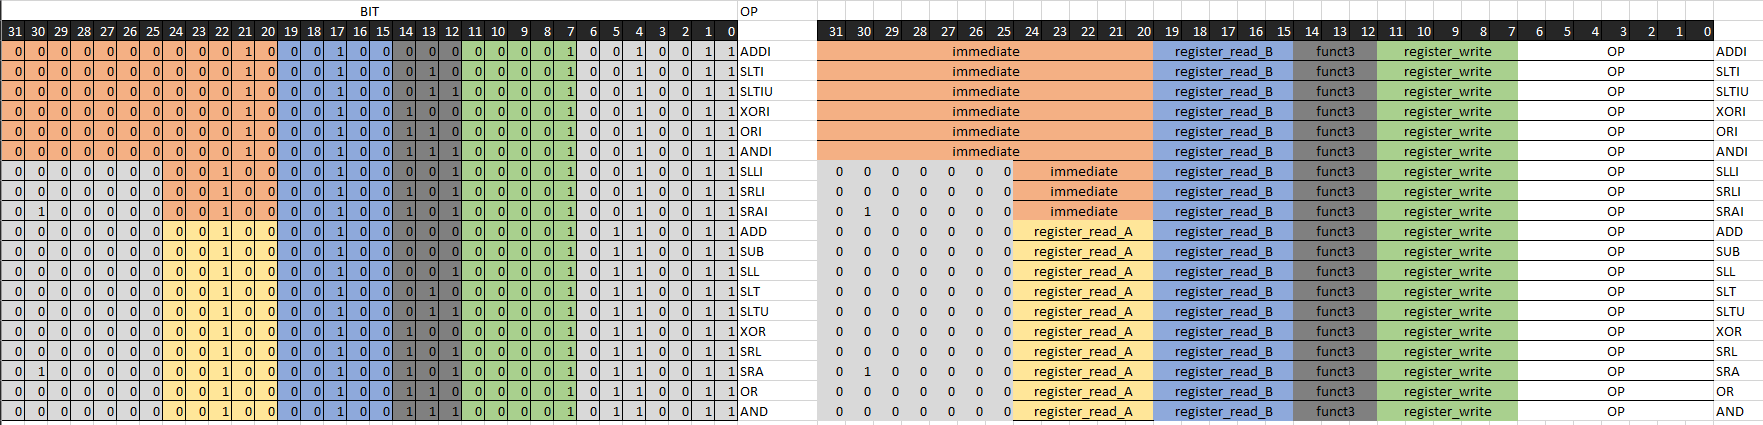
\includegraphics[width = 200mm,angle = 270, origin = c]{instruction_bits}
	\caption{Information extraction from 32-bit instruction word}
	\label{fig:instruction_bits}
\end{figure}


\section{Arithmetic Logical Unit}
The \acf{ALU} is the part of the processor that performs the arithmetic and logical operations. Figure \ref{fig:alu} gives an overview of what type of operations are performed.
\begin{figure}[H]
	\centering
	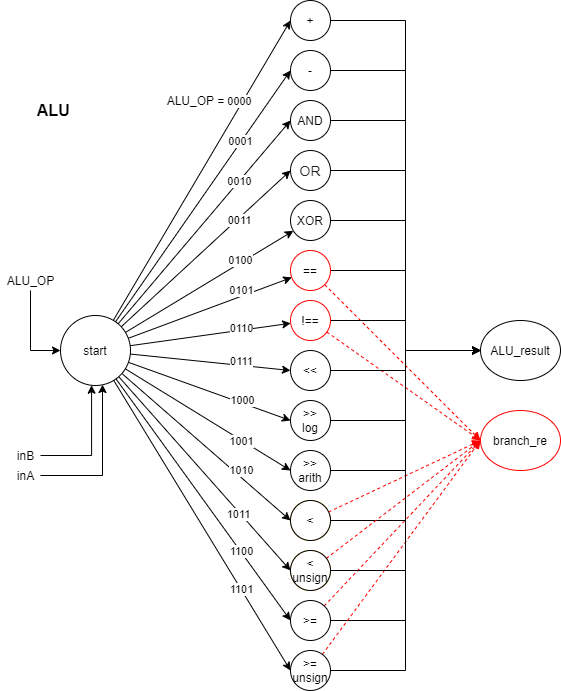
\includegraphics[width=\textwidth]{ALU.png}
	\caption{ALU operations}
	\label{fig:alu}
\end{figure}

\subsection{Architecture and Design}
To implement the ALU, it is required to have the data inputs as well as clock input and a control signal consisting of 4 bits to specify the required operation to be performed. Since there are instructions that require a branch response to know whether the next instructions shall be skipped or not, the ALU needs an additional output called \textit{branch\_re} other than the result output of the arithmetic/logical operation. The architecture of the ALU is shown in figure \ref{fig:alu_arch}:
\begin{figure}[H]
	\centering
	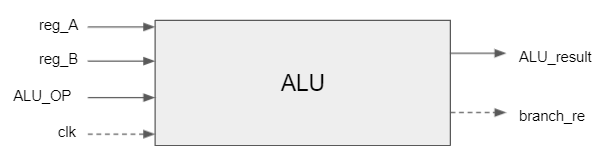
\includegraphics[width=\textwidth]{alu_arch.png}
	\caption{ALU operations}
	\label{fig:alu_arch}
\end{figure}
Not only the instructions e.g. \textit{ADD, SUB, XOR...} require an arithmetic operation but also \textit{LOAD, STORE..} require an ALU action. While \textit{ADD, SUB, XOR...} require an operation between the two input values (either register-register or register-immediate) to get a mathematical or logical result, the \textit{LOAD, STORE...} instructions require the ALU to build the target addresses for the memory access.
\subsection{Implementation}
The implementation of the ALU is based on figure \ref{fig:alu} and performs a switch-case on all the different input values of \textit{ALU\_OP}. The 4-bit input variable specifies the operation based on following declarations:
\begin{table}[H]
\setlength\arrayrulewidth{2pt}
\centering
	\begin{tabular}{|c|c|}
		\hline
		\rowcolor{light-gray}
		\textbf{ALU\_OP} & \textbf{Operation} \\
		\hline
		0000 & ADD \\
		\hline
		0001 & SUB \\
		\hline
		0010 & AND \\
		\hline
		0011 & OR \\
		\hline
		0100 & XOR \\
		\hline
		0101 & EQUAL \\
		\hline
		0110 & NEQUAL \\
		\hline
		0111 & shift\_left \\
		\hline
		1000 & shift\_right \\
		\hline
		1001 & shift\_right (arithmetic) \\
		\hline
		1010 & <\\
		\hline
		1011 & < (unsigned) \\
		\hline
		1100 & $\geq$ \\
		\hline
		1101 & $\geq$ (unsigned) \\
		\hline
	\end{tabular}
\caption{Input code and respective operation}
\end{table}
To visualize the implementation, a part of the VHDL code is displayed in the following. The case statement is based on the input \textit{alu\_op}. The ALU then performs the corresponding operation with the two inputs \textit{in\_a and in\_b}.\clearpage

\begin{lstlisting}[style=vhdl, caption=ALU VHDL code]
begin
	process(in_a, in_b, alu_op)
	begin
	--default output is 0
	branch_re <= '0';
	alu_result <= "00000000000000000000000000000000";	
		case alu_op is	
			when "0000" =>--"ADD"	
				alu_result <= in_b + in_a;	
			when "0001" =>--"SUB"	
				alu_result <= in_b -in_a;	
			when "0010" =>--"AND"	
				alu_result <= in_b AND in_a;
			when "0011" =>--"OR"
				alu_result <= in_b OR in_a;
			when "0100" =>--"XOR"
				alu_result <= in_b XOR in_a;
			when "0101" =>--"EQUAL"	
				if(in_b = in_a) then
				branch_re <= '1';
				else
				branch_re <= '0';
				end if;
	...
\end{lstlisting}
In case the operation determined by \textit{alu\_op} might be originating of a branch instruction, the \textit{branch\_re} flag has to be set respectively (line  19). Since the branch instructions only include some of the arithmetic and logical operations of the ALU, the default value for the \textit{branch\_re} is set as \textit{0}.

\clearpage
\section{\acf{RF}}
A register is a small memory element with high read and write speeds. It is therefore often used inside digital circuits to store data locally. In the case of a processor core, the total data stored in all registers specifies the machine state.\\
If the contents of each register are saved to some arbitrary memory the current state of the core can later be restored by loading this data to the corresponding registers. \\
The RISC-V unprivileged specification specifies 32 32-Bit general purpose register for the RV32I base instruction set \cite{riscv:unprivileged}.
To configure the core as well as storing status and general information about it multiple \acf{CSR} are introduced by the RISC-V privileged specification \cite{riscv:privileged}.\\
EDRICO implements both, all 32 32-Bit integer general-purpose registers as well as a selection of required \acp{CSR}.

\subsection{Architecture and Design}
A requirement for the Register Files is to allow access on one input data bus and two output data bus, each with a size of 32-Bit respectively. Multiple control signals can be accessed to control the data flow through the module. Registers are read asynchronously, hence a read operation is not dependent on any clock. Writes to a register are performed on a falling clock edge.\\
Some of the \acp{CSR} need to provide their contents to other modules without using one of the two designated output buses. This decreases unnecessary overhead on e.g. load and store operations. \\
Figure \ref{fig:RF_arch} depicts the architecture of the Register File module.

\begin{figure}[H]
	\centering
	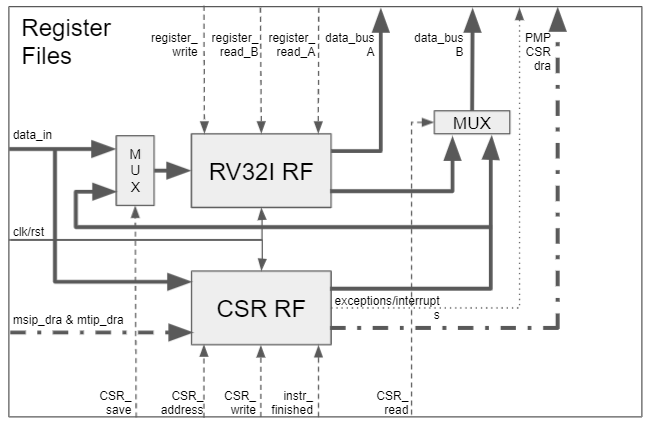
\includegraphics[width=\textwidth]{RF_arch.png}
	\caption{Register Files architecture}
	\label{fig:RF_arch}
\end{figure}

In order to write data to a register, the value needs to be put on the \textit{data\_in} bus and the corresponding control signals need to be configured. Data can be read either via the \textit{data\_busA} or \textit{data\_busB}, the CSR registers can only be accessed on \textit{data\_busB} via a MUX controlled by the \textit{CSR\_read} signal. If the bit is set, the CSR specified by \textit{CSR\_address} will be visible on \textit{data\_busB} at the next rising clock edge.\\
In order to store data to a CSR register, it has to be put on the \textit{data\_in} bus. If the \textit{CSR\_write} bit is set, the data is saved to the register specified by \textit{CSR\_address} on the next falling clock edge.\\
Execution of special \ac{CSR} instructions, like the Atomic Read/Write CSRRW \cite{riscv:unprivileged}, requires writing to both a general-purpose RV32I register and a \ac{CSR}. Since the control signals are not allowed to change during execution, it is mandatory to allow the \ac{CSR} \ac{RF} to write directly to the \ac{RV32I} \ac{RF} without utilizing the \textit{data\_in} bus.
In order to do so, the \textit{CSR\_save} signal is added to design. 
If it is applied, the \ac{CSR} Register File output is connected to the data input bus of the general purpose registers.  \\
Some of the \ac{CSR} allow direct memory accesses. These are implemented in a separate module, including the \textit{mtime}, \textit{mtimecmp} and \textit{msip} registers as well as a dedicated AXI4-Lite slave interface. To set the software and timer interrupt pending bits (which are caused by the memory mapped \ac{CSR}), the \textit{msip\_dra} and \textit{mtip\_dra} inputs are implemented.\\
The \ac{CSR} Register File is accessed by a 12 Bit addresses, \ac{RV32I} registers are accessed using a four byte address signal for each data bus, respectively.   
\subsubsection{General Purpose Registers}
The general purpose registers are used to store the data on which operations are performed on. Since RISC-V is a load-store architecture no data from the memory can be modified directly without loading it to a \ac{GPR} first (except when using atomic operations) \cite{riscv:unprivileged}.\\
Figure \ref{fig:gppr} shows the design of \ac{RV32I} Register File:
\begin{figure}[H]
	\centering
	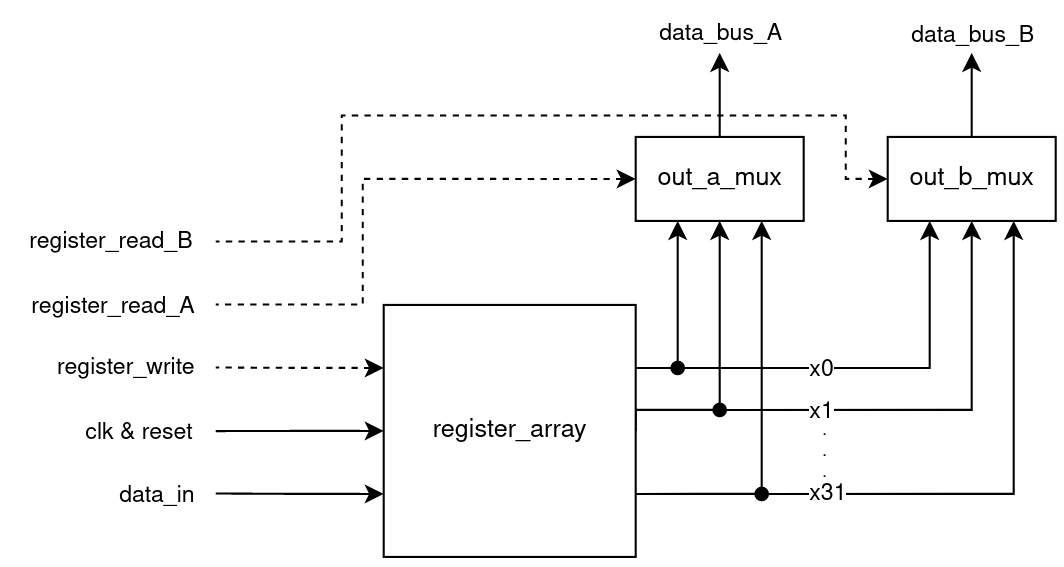
\includegraphics[width=\textwidth]{RV32I_new.png}
	\caption{General Purpose Registers}
	\label{fig:gppr}
\end{figure}
Every register may be modified via \textit{data\_in} and read via \textit{data\_busA} and \textit{data\_busB}.
The only limitation is \textit{x0}, per definition \textit{x0} must be hardwired to zero. Writing to the register is allowed but has no effect, reading will return \textit{0x00000000}.
According to the RV32I programmers model some of the other registers should be
used for dedicated purposes, like the stack pointer. There are no hardware checks
implemented in order to enforce those rules.\\
Writes are executed on a falling edge if the corresponding \textit{register\_write} signal is high. Reads are performed on a rising edge if the corresponding \textit{register\_read\_A/B} is high. There are no hardware checks implemented to prevent multiple registers from writing to the same data bus at the same time. This must be prevented by the controlling element e.g. the control unit.\\
All registers are cleared to \textit{0x00000000} on reset.
\subsubsection{\acf{CSR}}
CSRs are Control and Status Registers that are introduced to the design by the
RISC-V privileged specification. Some of the values stored inside the CSRs need to
be provided to the Exception Unit and the PMP \& PMA checker to decrease
complexity, some of that accesses can be performed through direct memory access.
Some of the CSRs are memory mapped. Memory mapped means they need to be
accessible via the system bus by any AXI4-Lite master. In order to implement this,
an AXI4-Lite salve module implementing all memory mapped CSRs is added to the
design.\\
Further Information about this module can be found in the chapter \ref{axi4slave}.
The CSRs that provide direct access are:
\begin{itemize}
	\item \textit{msip} and \textit{mtip} bits in the \textit{mpi} register (write)
	\item \textit{pmpcfg} (read)
	\item \textit{pmpaddress} (read)
\end{itemize}

Some registers are specified as WARL registers, meaning anything can be written to
them, but the value returned on read must be a legal value. Table \ref{table:csr} displays every non memory mapped CSR, the corresponding address, type, access possibility, width and a short description:
\begin{table}[H]
\setlength\arrayrulewidth{2pt}
\resizebox{\textwidth}{!}{
	\begin{tabular}{|>{\columncolor{light-gray}}l|>{\color{dark-green}}l|>{\color{dark-green}}l|>{\color{blue}}l|>{\color{red}}l|l|}
		\hline
		\rowcolor{light-gray}
		\textbf{register} & \color{black}\textbf{address} & \color{black}\textbf{type} & \color{black}\textbf{access} & \color{black}\textbf{width} & \textbf{description} \\
		\hline
		misa & 0x301 & WARL & R & 32-bit & describes supported ISAs \\
		\hline
		mvendorid & 0xF11 & N/A & R & 32-bit & describes vendor id
 \\
		\hline
		marchid & 0xF12 & N/A & R & 32-bit & describes architecture ID \\
		\hline
		mimpid & 0xF13 & N/A & R & 32-bit & describes implementation ID \\
		\hline
		mhartid & 0xF14 & N/A & R & 32-bit & describes hart id \\
		\hline
		mstatus & 0x300 & N/A & R/W & 32-bit & reflects \& controls a hart’s
		current operating state \\
		\hline
		mtvec & 0x305 & N/A & R/W & 32-bit & holds trap vector configuration \\
		\hline
		mie & 0x304 & N/A & R/W & 32-bit & reflects interrupt enable state \\
		\hline
		mip & 0x344 & N/A & R & 32-bit & holds interrupt pending bits \\
		\hline
		mcycle & 0xB00 & N/A & R/W & 64-bit & holds count of clock cycles \\
		\hline
		minstret & 0xB02 & N/A & R/W & 64-bit & holds count of executed
		instructions \\
		\hline
		mhpcounter(3-31) & 0xB03-0xB1F & N/A & R/W & 32-bit & holds count of events (lower 32
		bit) \\
		\hline
		mhpcounterh(3-31) & 0xB83-0xB9F & N/A &  & 32-bit & holds counter of events (upper
		32 bit) \\
		\hline
		mhpevent(3-31) & 0x323-0x33F & N/A & R/W & 32-bit & specifies events on which to increment corresponding
		mhpmcounter
 \\
		\hline
		mcountinhibit & 0x320 & WARL & R/W & 32-bit & controls which hardware
		performance monitoring
		counters increment \\
		& & & & & (if set, no increment) \\
		\hline
		mscratch & 0x340 & N/A & R/W & 32-bit & Dedicated for use by
		machine-mode
 \\
		\hline
		mepc & 0x341 & WARL & R/W & 32-bit & holds jump-back address during
		interrupt
 \\
		\hline
		mcause & 0x343 & N/A & R/W & 32-bit & specifies cause of
		exception/interrupt \\
		\hline
		mtval &  & N/A & R/W & 32-bit & holds information about trap \\
		\hline
		pmpcfg0-3 & 0x3A0-0x3A3 & N/A & R/W & 32-bit & Physical memory protection
		configuration
 \\
		\hline
		pmpaddr0-15 & 0x3B0-0x3BF & N/A & R/W & 32-bit & Physical memory protection
		address register \\
		\hline
	\end{tabular}}
\label{table:csr}
\caption{List of implemented CSRs}
\end{table}
\clearpage
The architecture of the CSR Register File is shown in \ref{fig:csrarch}.
\begin{figure}[H]
	\centering
	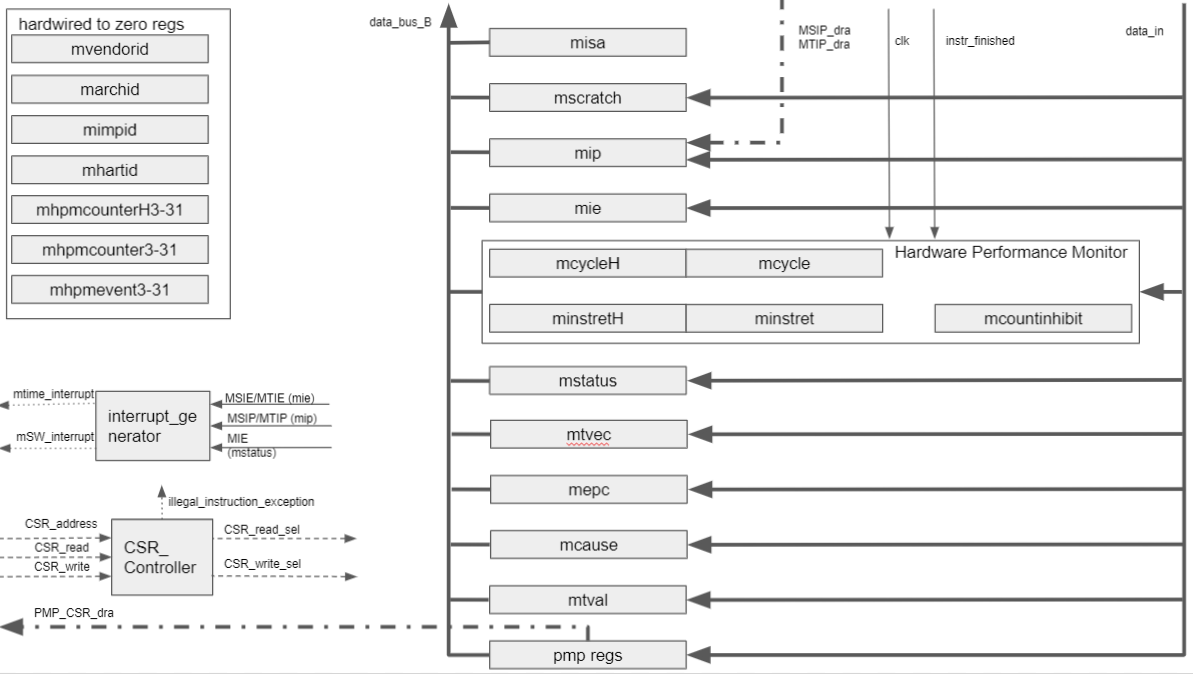
\includegraphics[width=\textwidth]{csrreg.png}
	\caption{CSR Register File Architecture}
	\label{fig:csrarch}
\end{figure}
The CSR Register File is comprised of the different CSR Registers, \textit{CSR\_Controller} and \textit{interrupt\_generator}.\\
Some of the implemented CSR registers are hardwired to zero, reads to those addresses return \textit{0x00000000} and writes have no effect if the register is defined as read only the write will result in an \textit{illegal\_instruction\_exception}. Other CSR registers may be defined as read-only. \\
The \textit{CSR\_Controller} checks if a CSR access is allowed and produces access signals for each register from the given address. If an address is not writable but yet a write is requested, the \textit{CSR\_Controller} raises an \textit{illegal\_instruction\_exception}.\\
The \textit{interrupt\_generator} checks if an interrupt is pending, enabled and if interrupts are globally enabled. In that case the corresponding interrupt is raised. The interrupts remain pending, as long as the corresponding direct register access signals it. To prevent the machine from being stuck in the interrupt, the programmer of the \ac{ISR} must clear the pending interrupts, e.g. the timer interrupt by writing to the memory mapped CSRs.\\
Some registers have special functionalities. The Hardware Performance Monitor for example counts the number of clock cycles as well as the number of executed instructions. Calculation of the \ac{CPI} can be performed as shown in \eqref{eq:CPI}:

\begin{align}
	CPI=\frac{mcycleH>>32+mcylce}{minstretH>>32+minstret}\label{eq:CPI}
\end{align}

During Benchmarks these registers can be used to calculate the performance of the core.\\
For physical memory protection, several attributes such as read and write can be specified inside the \ac{PMP} \ac{CSR}, a more detailed description of these specific registers can be found in: \cite{riscv:privileged}.\\
There are 16 \textit{pmpaddr} and four \textit{pmpcfg} registers. In order to verify that a memory access does not violate any \ac{PMP} rules, the PMP and PMA checker needs access to these registers. Performing this accesses over the \textit{data\_out\_B} bus would result in 16+4 data transfers, so 20 register accesses in total. This would impose a significant overhead of at least 20 clock cycles on every memory access. To reduce the effect of checking the \ac{PMP} rules a direct register access is implemented. 
\subsection{Implementation}
Implementing the \ac{RV32I} \ac{RF} is done by defining an array of 32 \textit{std\_logic\_vector} of 32-Bit each. The zeroth element in the array corresponds to the x0 register, therefore it can not be written and is hardwired to zero.\\
On a write, the 5-Bit \textit{register\_write} signal is used to index the corresponding array element. This is only possible since writes to the x0 register do not effect the state of the machine. Hence, no writes are performed if the write signal is set to \textit{0b00000}.\\
Since some \ac{CSR} have additional features they need to be implemented individually, therefore the matrix approach used for the \ac{RV32I} register files can not be taken. There are multiple registers that are hardwired to zero, they are implemented as one and the read write multiplexers access the same register if an access to one of these registers occurs.\\
To safe resources all \ac{CSR} implement just the bits that are needed, the others are hardwired to zero. The following listing illustrates this concept, using the \textit{mstatus} register as an example, figure \ref{fig:mstatus} shows the mstatus register according to \cite{riscv:privileged}:

\begin{figure}[H]
	\centering
	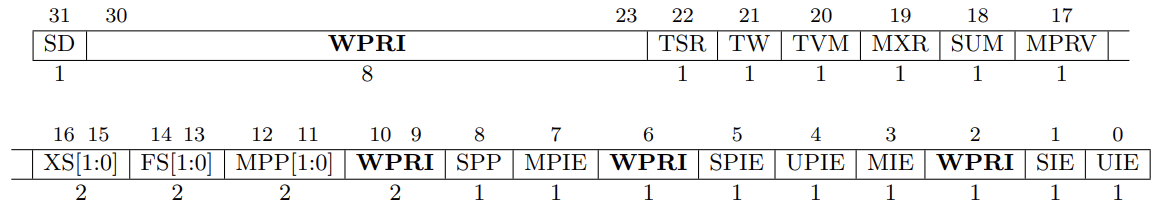
\includegraphics[width=\textwidth]{mstatus.png}
	\caption{32-Bit machine mode register (\textit{mstatus}) \cite{riscv:privileged}}
	\label{fig:mstatus}
\end{figure}

\begin{lstlisting}[style=vhdl, caption=mstatus implementation]
	---------------------------------------------------------
	--mstatus register
	---------------------------------------------------------
	mstatus_proc: process(reset, clk)
	begin
	if(reset = '1') then
	mstatus_reg <= (others => '0');
	elsif(clk'event and clk = '0' and write(0) = '1') then
	mstatus_reg <= data_in(7) & data_in(3);
	end if;
	end process;
	
	mstatus <= x"000018" & mstatus_reg(1) & "000" & mstatus_reg(0) & "000";
\end{lstlisting}

For the chosen implementation only two bits in the status register are relevant, \ac(MPIE) and \ac{MIE}. Every Other bit can be hardwired to a specific value. Since neither supervisor nor user mode are implemented are the corresponding (prior) interrupt enable bits tied to zero. The \textit(xPP) fields hold the previous privilege mode in which the machine was prior to a trap. Only machine mode is implemented, hence \ac{MPP} can be hardwired to "11" and \ac{SPP} to "00". According to \cite{riscv:privileged} all other bits may be hardwired to zero if only machine mode is implemented. \\

\section{PMP and PMA Checker}
Physical memory protection and attribute checking must be done in
order to ensure that only allowed and defined memory regions are accessed, providing
minimum of security and preventing the core from accessing not defined regions, which
may result in the core getting stuck.\\


\subsection{Architecture and Design}
An overview of the \ac{PMP} \& \ac{PMA} Checker is illustrated by \ref{fig:pmparch}:

\begin{figure}[H]
	\centering
	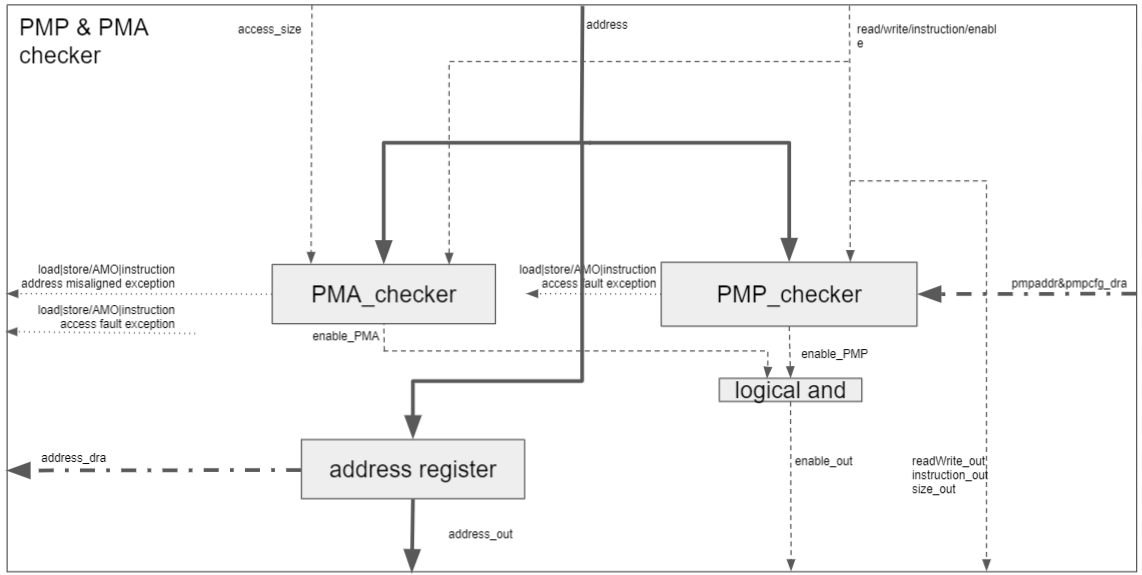
\includegraphics[width=\textwidth]{pmparch.png}
	\caption{PMP \& PMA Checker Architecture}
	\label{fig:pmparch}
\end{figure}

The \textit{PMP\_checker} is used to define memory regions and enforce several rules onto
those, for example if instructions may be fetched from a region or if writes are
allowed. In order to apply the rules the corresponding region must be locked by
setting the L-bit inside the corresponding \textit{pmpcfg} \ac{CSR}. Once locked, regions may only be unlocked by a system reset. After a restart every region is unlocked and
reset, e.g. a boot loader could enforce several rules for memory accesses in M-Mode before control hand-over to the main software running on the core. If a \ac{PMP} entry is not locked, every memory access that matches this address space succeeds.
\\
In order to specify, if reads, writes or instruction fetches are possible to a certain address, it needs to be specified inside the \textit{pmpaddr} and corresponding \textit{pmpcfg} CSRs. If an address is not specified every access is allowed, as long as the hart operates in machine mode. The PMP unit has direct access to those and enforces the rules. Figure \ref{fig:pmpaddr} and \ref{fig:pmpcfg} show these two registers.\\

\begin{figure}[H]
	\centering
	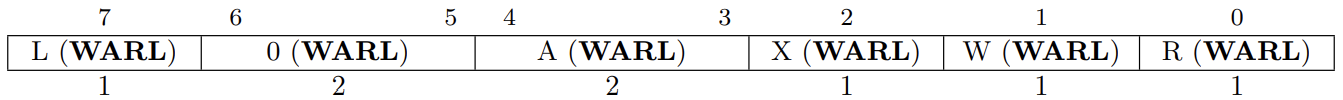
\includegraphics[width=\textwidth]{pmpcfg.png}
	\caption{8 Bit from 32-Bit \textit{pmpcfg} register \cite{riscv:privileged}}
	\label{fig:pmpaddr}
\end{figure}


\begin{figure}[H]
	\centering
	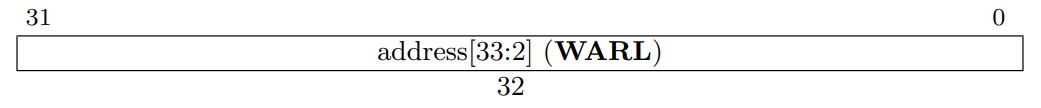
\includegraphics[width=\textwidth]{pmpaddr.png}
	\caption{\textit{pmpaddr} register \cite{riscv:privileged}}
	\label{fig:pmpcfg}
\end{figure}

One \textit{pmpcfg} register is comprised of four 8-bit configuration fields, one of which is shown in \ref{fig:pmpcfg}. The X, W and R bit specify whether or not the region defined by this entry is fit for instruction accesses, reads or writes. The size and range of the region is specified by the mode chosen by setting the A field in the configuration register. It can be configured to disable the region, specify it as \ac{TOR}, \ac{NA4} or \ac{NAPOT}. 

Right now there is a single PMA check implemented, its job is to check if the memory
access is aligned. A word is 32-bit, halfword 16-bit and byte 8-bit. The smallest
addressable data unit is one byte long. Therefore a word access is aligned, if the
memory address modulo 4 is 0 (two LSBs are zero), for a halfword access the
memory address modulo 2 must be zero (LSB is zero) and byte accesses are allowed
on every address.
\\
For both units (PMP and PMA) information about the access like the access size
and type must be provided, this is done by the control unit. PMP and PMA checks
are applied on the data present as soon as the enable signal is applied. Both checks
are simple logical functions and must be performed under a clock cycle. The address
register is updated with the corresponding address after every PMP, independent of
its result. This must be done since the Exception Control needs access to the faulty
address at the rising clock edge if an exception is risen.
\\
The logical and is used, in order to ensure that both the \textit{PMA\_checker} and
\textit{PMP\_checker} rules are enforced.
\subsection{Implementation}

\section{Exception Control}
The Exception Control Unit is used to guard exception entries and exits one of its
tasks is e.g. to modify the PC accordingly and save information about the exception.
In addition, two interrupt entries are guarded by the unit. A list of all supported
exceptions and interrupts is listed below:\\
Exceptions can be caused by the following modules:
\begin{itemize}
	\item Control Unit
	\item CSR register file
	\item PMP \& PMA checker
\end{itemize}

The Control Unit may cause the following exceptions:
\begin{itemize}
	\item illegal instruction exception
	\item breakpoint exception
	\item environment-call-from-M-mode exception
\end{itemize}

The PMP \& PMA checker may cause the following exceptions:
\begin{itemize}
	\item load access fault exception
	\item store/AMO access fault exception
	\item instruction access fault exception
	\item load address misaligned exception
	\item store/AMO address misaligned exception
	\item instruction address misaligned exception
\end{itemize}

The CSR register file may cause the following exceptions/interrupts:
\begin{itemize}
	\item timer interrupt
	\item software interrupt
	\item illegal instruction exception
\end{itemize}
\subsection{Architecture and Design}
Figure \ref{fig:EC} shows the architecture of the Exception Control:
\begin{figure}[H]
	\centering
	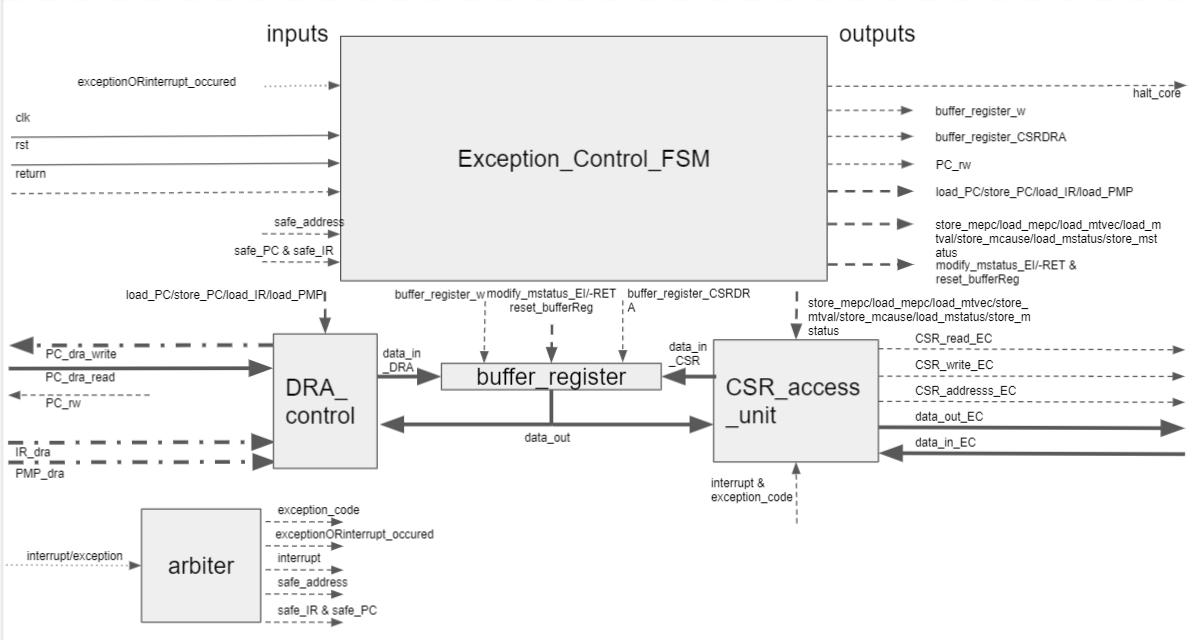
\includegraphics[width=\textwidth]{EC.png}
	\caption{Exception Control Architecture}
	\label{fig:EC}
\end{figure}
The Exception Control module is comprised of a FSM, an arbiter to decide if an
interrupt or exception is taking place and which one shall be handled if multiple are raised at a time. To modify registers a \textit{DRA\_control} as well as a \textit{CSR\_access\_unit} and a buffer register are added to the design.\\
The arbiter receives the different exception and interrupt signals, it’s purpose is to decide which interrupt will be executed and generate the according exception code
as well as the signal for the FSM to start the routine.\\
The \textit{DRA\_control} module is used to load the Instruction Register, PMP address register and Program Counter. A load to the PC may also be performed, in order to do so the \textit{PC\_rw} signals must be asserted one clock cycle earlier by the FSM.\\
The \textit{buffer\_register} is implemented to allow data shares between the \textit{DRA\_control} and \textit{CSR\_access\_unit}. It implements another functionality that allows to set either the MIE register to 1 (exit) or the MPIE register to 0 (entry) and switch the two bits (MIE and MPIE) on the \textit{data\_out} line. This feature is used during the phase of modifying the \textit{mstatus} register and allows the modify to happen in at least two clock
cycles.\\
The \textit{CSR\_access\_unit} is used to perform register accesses to the CSR register file. During Exception entry or return the data bus B must be connected to the
\textit{data\_in\_EC} bus and the \textit{data\_in} bus to the \textit{data\_out\_EC} bus. This is done by implementing a multiplexer at the corresponding buses controlled by the\textit{ halt\_core} signal.\\
If an Exception or Interrupt is raised, the Exception Control unit must write the
current \textit{PC+4} to the \textit{mpec} register, modify the \textit{mcause} register to reflect the cause of the exception/interrupt and update the \textit{mtval} CSR to provide additional information on the taken trap. If multiple exceptions occur at once, only the highest priority exception is taken.\\
If an Exception is raised, while the processor is handling another exception, \textit{mpec}, \textit{mcause} \& \textit{mtval} are overwritten. The saving of the return address and other information stored in those registers is left to the trap handler, in order to avoid a large hardware register stack.\\
If an exception entry is performed the \textit{exceptionORinterrupt\_occured} signal on the FSM is high, if the return signal is high it indicates that an exit shall be performed, however if both signals are high (should not happen in normal operation) the entry will be performed.

\subsection{Implementation}

\section{AXI4-Lite Master}
To connect the processor to peripherals the AXI4-Lite protocol is used. Due to its
popularity many IPs such as BRAM can be connected to each other using an
Interconnect. EDRICO contains a Master and a Slave interface. Both of which are
explained in more detail in the following sections:
\subsection{Architecture and Design}
The AXI4-Lite Master is implemented in order to allow memory accesses e.g. to a
BRAM or UART IP. The following figure depicts the architecture of the master:
\begin{figure}[H]
	\centering
	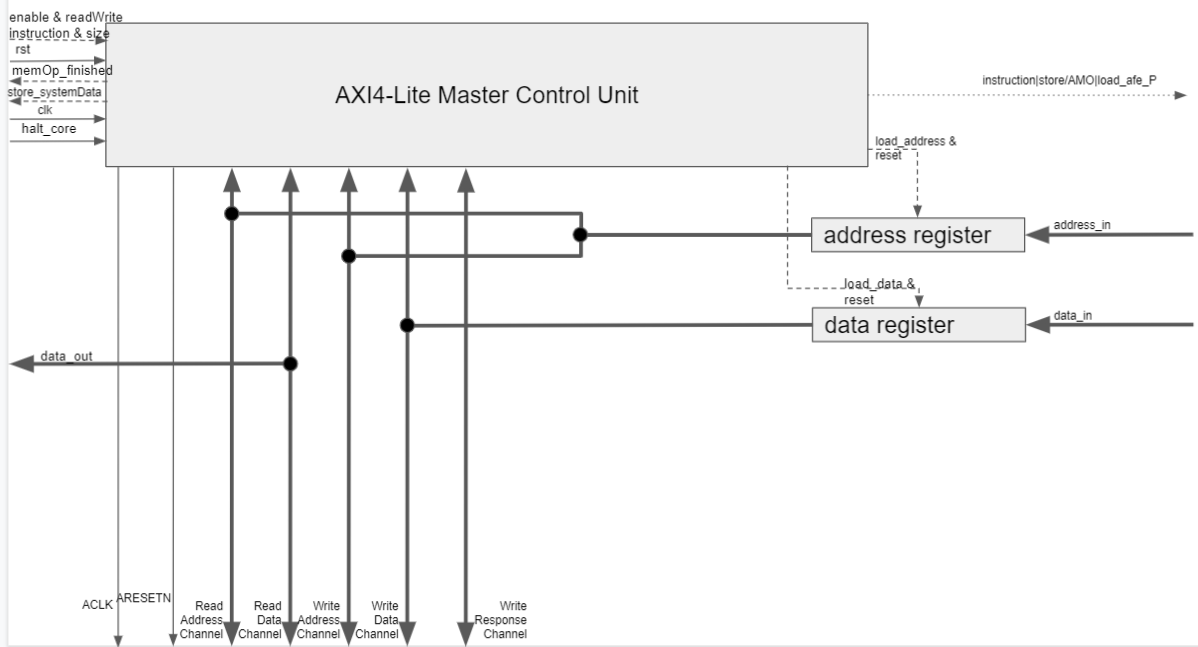
\includegraphics[width=\textwidth]{aximaster.png}
	\caption{AXI4-Lite Master Architecture}
	\label{fig:aximaster}
\end{figure}
It includes two registers, the data register and the address register, these are loaded on the rising edge of the system clock if the corresponding load signal is applied. Both register outputs are constantly applied to the corresponding AXI signals \textit{(AWADDR, ARADDR and WDATA)}.\\
The AXI4-Lite Master Control Unit is in charge of controlling the AXI Transfer. It
controls the ready and valid signals as well as the register reads and writes. It is
clocked with \textit{clk}. The \textit{rst} signal will reset it. The Master also provides the clock and reset for every slave connected to the AXI interconnect. To start a transfer, the enable signal must be high on a rising edge of the clock, in that case the address and data register are loaded on the next falling edge of system clock.\\
If data is ready to be read from the system bus, it is routed to an output of the Master and the \textit{store\_systemSystemData} is set to high, in order to ensure a correct read, this process shall not be clocked. The surrounding system must then process these signals to store the data in the correct register.\\
At the end of a data transfer, the \textit{memOp\_finished} signal is set to high and remains high until a new transfer is initiated.\\
If an error occurred during an access, the \textit{instruction\_afe\_P}, \textit{storeAMO\_afe\_P} or \textit{load\_afe\_P} exceptions are raised. And remain high until the \textit{halt\_core} signal is applied to the AXI4-Lite Master Control Unit.
\subsection{Implementation}

\section{AXI4-Lite Slave}
\label{axi4slave}
Some of the RISC-V CSRs must be memory mapped, meaning the must be
accessible by other devices via the memory space. The addresses can be specified
by setting a generic in the VHDL code. A basic address is predefined for each CSR,
corresponding to the CLINT module by sifive since this is the closest thing to industry
standard.
\begin{table}[H]
	\setlength\arrayrulewidth{2pt}
	\centering
	\resizebox{\textwidth}{!}{
	\begin{tabular}{|>{\columncolor{light-gray}}l|>{\color{dark-green}}l|>{\color{blue}}l|>{\color{red}}l|l|}
		\hline
		\rowcolor{light-gray}
		\color{black}\textbf{register} & \color{black}\textbf{address} & \color{black}\textbf{access} & \color{black}\textbf{width} & \color{black}\textbf{description}\\
		\hline
		msip & 0x0200\_0000 & R/W & 32-bit & hold software interrupt pending bit \\
		\hline
		mtimecmp & 0x0200\_4000 & R/W & 32-bit & hold time compare value (lower 32 bit) \\
		\hline
		mtimecmph & 0x0200\_0004 & R/W & 32-bit & hold time compare value (upper 32 bit) \\
		\hline
		mtime & 0x0200\_BFF8 & R/W & 32-bit & hold time (lower 32 bit) \\
		\hline
		mtimeh & 0x0200\_BFFB & R/W & 32-bit & hold time (upper 32 bit) \\
		\hline
	\end{tabular}}
	\caption{Memory Mapped CSRs}
\end{table}
\subsection{Architecture and Design}
The AXI4-Lite slave is in charge of accepting data transfers and reading/writing the
CSRs. Figure \ref{fig:axislave} shows the architecture, including the memory mapped CSRs:
\begin{figure}[H]
	\centering
	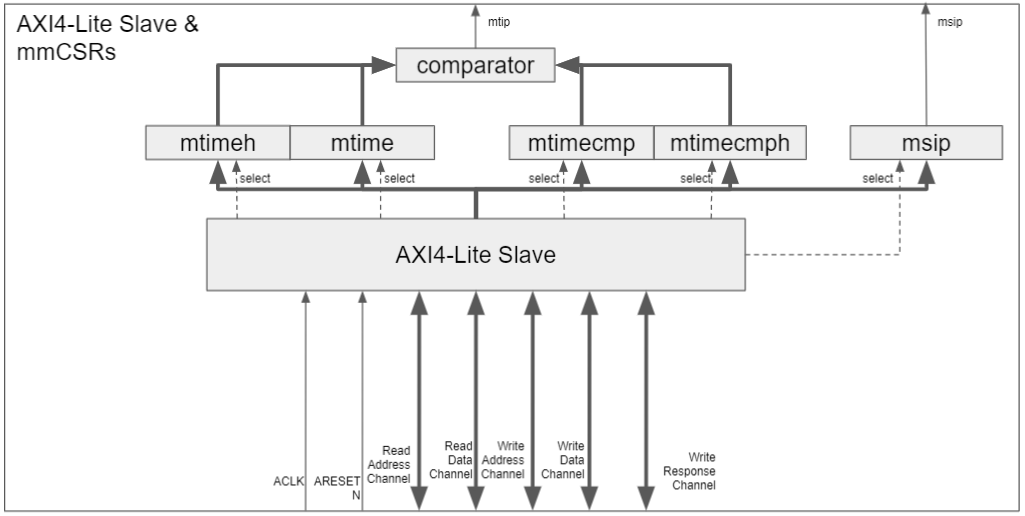
\includegraphics[width=\textwidth]{axislave.png}
	\caption{AXI4-Lite Slave Architecture}
	\label{fig:axislave}
\end{figure}
As an AXI4-Lite slave an IP core may be used. In fact the Vivado AXI Interface
generator may be used to generate the AXI4-Lite Slave as well as the registers, this
IP could then be modified with the comparator and the \textit{msip} and \textit{mtip} output
The AXI Slave allows reads and writes to the 32 bit registers \textit{mtimeh}, \textit{mtime},
\textit{mtimecmp} and \textit{mtimecmph} and the one byte \textit{msip} register.\\
The comparator is used to trigger a timer interrupt. It compares \textit{mtime} and
\textit{mtimecmp}. If the value of \textit{mtime} is equal or greater than the one in \textit{mtimecmp}, the
\textit{mtip} signal is asserted.\\
The interrupt remains posted, until it is cleared by writing to the \textit{mtimecmp} register.
The \textit{msip} register is a one byte register, the remaining 31 bits are hardwired to zero.
Its reset value is zero. If it is set to one, the \textit{msip} bit in \textit{mip} is set and therefore, a
software interrupts may be risen.\\
Table \ref{CSRreset} shows the reset values for each CSR:
\begin{table}[H]
	\setlength\arrayrulewidth{2pt}
	\centering
	\begin{tabular}{|>{\columncolor{light-gray}}l|l|}
		\hline
		\rowcolor{light-gray}
		\textbf{register} & \textbf{value} \\
		\hline
		msip & '0' \\
		\hline
		mtimeh & 0x00000000 \\
		\hline
		mtime & 0x00000000 \\
		\hline
		mtimecmph & 0xFFFFFFFF \\
		\hline
		mtimecmp & 0xFFFFFFFF \\
		\hline
	\end{tabular}
	\label{CSRreset}
	\caption{Memory Mapped CSRs reset values}
\end{table}
\subsection{Implementation}
